\usetikzlibrary{positioning, chains, shapes.geometric, fit, shapes, arrows.meta, calc, backgrounds}

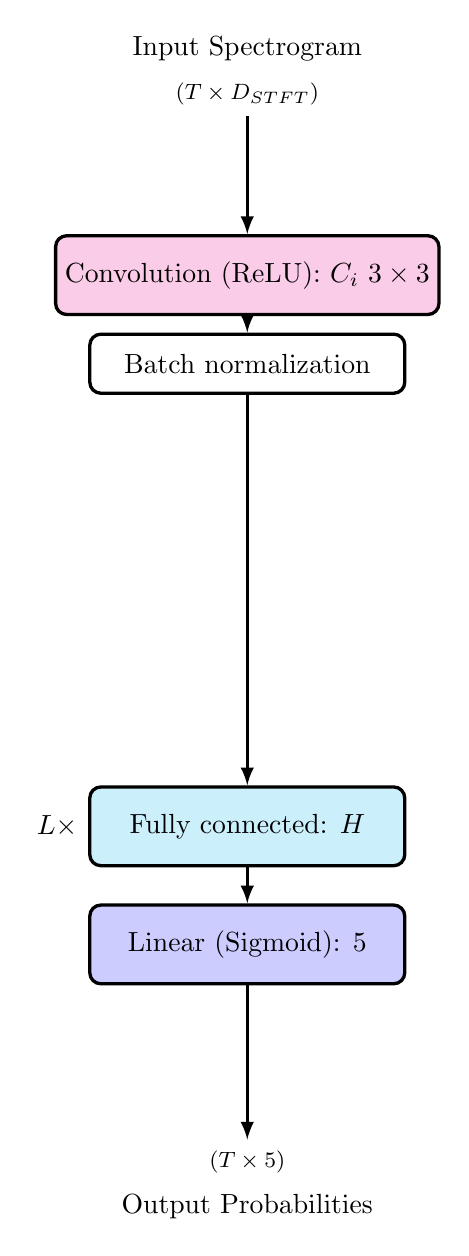
\begin{tikzpicture}[
    very thick,
    arrow/.style={
        -latex,
        very thick,
        rounded corners=0.2cm
    },
    ]

\node[anchor=south, label=above:{Input Spectrogram}] at (0, 0){\footnotesize{($T \times D_\text{STFT}$)}};

\draw[arrow] (0, 0) -- (0, -1.5) node [rectangle,
rounded corners,
draw,
anchor=north,
fill=magenta!20,
minimum height=1cm,
minimum width=4cm
] (a) {Convolution (ReLU): $C_i$  $3 \times 3$};

\draw [arrow] (a) -- (0, -2.75) node[rectangle,
rounded corners,
draw,
anchor=north,
fill=white!100,
minimum height=0.75cm,
minimum width=4cm
] (b) {Batch normalization};

\draw[arrow] (b) -- (0, -8.5) node[rectangle, 
rounded corners, 
draw, 
anchor=north, 
label=west:$L\times$,
fill=cyan!20,
minimum height=1cm,
minimum width=4cm
] (g) {Fully connected: $H$};

\draw[arrow] (g) -- (0, -10) node[rectangle, 
rounded corners, 
draw, 
anchor=north, 
fill=blue!20,
minimum height=1cm,
minimum width=4cm
] (h) {Linear (Sigmoid): $5$};

\draw[arrow] (h) -- (0, -13);

\node[anchor=north, label=below:{Output Probabilities}] at (0, -13){\footnotesize{($T \times 5$)}};

\end{tikzpicture}